\documentclass{article}
\usepackage{amsmath,amsthm,amsfonts,amssymb,fullpage,graphicx}

\begin{document}
\begin{flushleft}

\Large

Sheet 23: Graphs\newline

\normalsize



\textbf{Definition 1}
\textsl{A simple graph is a tuple $(V,E)$ where $V$ is a set and $E$ is a symmetric relation on $V$ without loops, that is, for all $x \in V$, $(x,x) \notin E$. Elements of $V$ are called vertices and unordered pairs $(x,y) \in E$ are called edges.}\newline

\textbf{Definition 2}
\textsl{Let $(V,E)$ be a simple graph. We say that $x \in V$ is a neighbor of $y \in V$ if $(x,y)$ is an edge. The degree of a vertex $v \in V$ is defined to be the number of neighbors of $v$.}\newline

\textbf{Exercise 3}
\textsl{There was a casual chess afternoon in class. Every two students played at most once with each other. Show that there are necessarily two students who played the same number of games. Is this true for infinite simple graphs?}
\begin{proof}
Assume to the contrary that no two students played the same number of games. Then every student played a different number of games. If there are $n$ students, then we see that no student can play more than $n-1$ games since there are $n$ people and a student can't play himself. So one student played $0$ games, one played $1$ game, etc. and one student played $n-1$ games. But since no student played another student more than once, then the student who played $n-1$ games must have played every student in the room other than himself. This includes the student who played $0$ games. This is a contradiction.
\end{proof}

\textbf{Exercise 4}
\textsl{There is a party at Marcello's with $19$ people attending. Is it possible that everyone knows exactly $3$ other people?}\newline

No
\begin{proof}
Suppose that there exists a graph with $19$ vertices, all of degree $3$. Then if we sum the degrees of every vertex we should end up with twice the number of edges there are in the graph, since edges are a symmetric relation. But $19\cdot 3 = 39$ is an odd number. Thus there does not exist such a graph.
\end{proof}

\textbf{Exercise 5}
\textsl{How about $n$ people attending?}
\begin{proof}
If $n$ is odd then a similar argument as used in Exercise 4 will show that it's impossible. If $n$ is even then make a graph with two sets of $n/2$ vertices, each arranged in a ring. Then within each ring every vertex has degree $2$ and since there are the same number of vertices in each ring we can connect each element of one ring to a unique element in the other so that each vertex in the graph has degree $3$. Thus there exists a graph where everyone knows exactly three people.
\end{proof}

\textbf{Exercise 6}
\textsl{A triangle is a set of $3$ vertices such that every pair is an edge. An empty triangle is a set of $3$ vertices with no edges. Draw a graph on $5$ vertices with no triangles or empty triangles.}\newline

\begin{center}
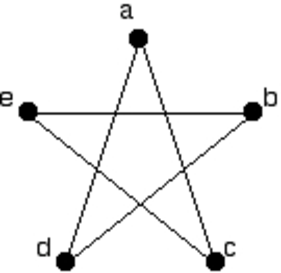
\includegraphics{star}
\end{center}

\textbf{Exercise 7}
\textsl{Show that every simple graph on $6$ vertices contains a triangle or an empty triangle.}
\begin{proof}
Let the $6$ vertices be $a$, $b$, $c$, $d$, $e$ and $f$. We see that, $a$ must have $3$ neighbors or not have $3$ neighbors since there are five other vertices. Consider the case where vertex $a$ has three neighbors. Without loss of generality let them be $b$, $c$ and $d$. If any of $b$, $c$ or $d$ are neighbors, then together with $a$ there exists a triangle. But if none of $b$, $c$ and $d$ are neighbors then those three make an empty triangle. Similarly, if $a$ is not neighbors with $b$, $c$ and $d$, then if any of $b$, $c$ and $d$ aren't neighbors we have an empty triangle. But if $b$, $c$ and $d$ are all neighbors then they form a triangle. In all cases there exists a triangle or an empty triangle.
\end{proof}

\textbf{Exercise 8}
\textsl{Show that in every simple graph the number of vertices of odd degree is even.}
\begin{proof}
Let $(V,E)$ be a graph and let $a$ be the number of vertices with even degree and $b$ be the number of vertices of odd degree. Also let $x$ be the sum of the degrees of vertices with even degree and $y$ be the sum of degrees of vertices with odd degree. Note that $x+y$ should be twice the number of edges in $(V,E)$ since $E$ is a symmetric relation and we don't allow loops. Thus $x+y=2k$ with $k \in \mathbb{Z}$. Note that regardless of the parity of $a$, $x$ must be even since it is the sum of even degrees. Thus $x = 2l$ for $l \in \mathbb{Z}$ and so $y = 2k-2l = 2(k-l)$ and since $k-l \in \mathbb{Z}$ we have $y$ is even. But then since $y$ is the sum of odd degrees, $b$ must be even, otherwise $y$ would be the odd sum of odd degrees and be odd.
\end{proof}

\textbf{Exercise 9}
\textsl{What does a graph such that every vertex has degree $2$ look like?}
\begin{proof}
Let $(V,E)$ be a finite graph with $n$ vertices such that each vertex has degree $2$. Note that the smallest $n$ can be is $3$, so let there be $3$ vertices, $a$, $b$ and $c$. We have $a$ has degree $2$ so $(a,b), (a,c) \in E$ and $b$ has degree $2$ so $(b,c) \in E$. Note that the edges for $c$ are accounted for and so $(V,E)$ must be a triangle for $n=3$. Use induction on $n$ and suppose that for a graph $(V,E)$ with $n$ vertices such that each vertex has degree $2$, one connected component is a polygon. Now let $|V| = n+1$. Consider one vertex, $a$, and consider the graph without $a$ or the two edges attached to it and instead, an edge connecting the two neighbors of $a$. Then this graph has $n$ vertices each with degree $2$, so each connected component is a polygon. But then in the original graph there was a connected component containing $a$ which was a polygon.\newline

Now suppose that $(V,E)$ is an infinite graph such that each vertex has degree $2$. Take some vertex and label it $a_0$. Arbitrarily label it's neighbors $a_1$ and $a_{-1}$. Then the other neighbors of $a_1$ and $a_{-1}$ are $a_2$ and $a_{-2}$ respectively. Continue in this way so that each vertex is labeled according to one of its neighbors and the whether the index of that vertex is positive or negative. There are two possibilities. First suppose that we reach a vertex that is already labeled. Then there are finitely many points making a cycle which means we have a connected component which is a polygon. The second case is that a vertex never gets labeled. Then this vertex isn't connected to the vertices getting labeled. Thus, the connected components of $(V,E)$ are either finite polygons or infinite lines of vertices.
\end{proof}

\textbf{Definition 10}
\textsl{Let $(V,E)$ be a graph. A walk of length $n$ from $x \in V$ to $y \in V$ is a sequence of vertices $a_0, a_1, \dots ,a_n$ where $a_0 = x$, $a_n = y$ and $(a_i, a_{i+1}) \in E$ $(0 \leq i \leq n-1)$. A path is a walk such that $a_i \neq a_j$ $(0 \leq i < j \leq n)$. A cycle is a walk such that $a_0 = a_n$ and $a_i \neq a_j$ $(0 \leq i < j \leq n)$.}\newline

\textbf{Theorem 11}
\textsl{If there is a walk from $a$ to $b$ there is a path from $a$ to $b$.}
\begin{proof}
Let $W = \{a_0, a_1, \dots , a_n\}$ such that $a_0 = a$ and $a_n = b$ be the shortest walk from $a$ to $b$. Suppose that $a_i = a_j$ for some $0 \leq i < j \leq n$. Then $W' = \{a_0, a_1, \dots , a_i, a_{j+1}, \dots , a_n\}$ is also a walk from $a$ to $b$ which is shorter than $W$. This is a contradiction and so for all $a_i, a_j \in W$ we have $a_i \neq a_j$. Thus $W$ is a path from $a$ to $b$.
\end{proof}

\textbf{Theorem 12}
\textsl{Let $\sim$ be a relation on $V$ where $a \sim b$ if there is a walk from $a$ to $b$. Then $\sim$ is an equivalence relation.}
\begin{proof}
Let $(V,E)$ be a graph and let $a,b,c \in V$. We have $a \sim a$ because of the walk of length $0$. Now let $a \sim b$. Then there exists a walk $W = \{a_0, a_1, \dots , a_n\}$ such that $a=a_0$ and $b=a_n$. Since $W$ is a walk, $(a_i, a_{i+1}) \in E$ for all $1 \leq i \leq n-1$. But then since $E$ is a symmetric relation we have $(a_{i+1}, a_i) \in E$ for all $1 \leq i \leq n-1$. Thus there exists a walk $W' = \{a_n, a_{n-1}, \dots , a_1\}$ from $b$ to $a$ and $b \sim a$. Finally suppose that $a \sim b$ and $b \sim c$. There there exists walks $W_1 = \{a_0, a_1, \dots , a_n\}$ and $W_2 = \{b_0, b_1, \dots , b_m\}$ with $a = a_0$, $b = a_n = b_0$ and $c = b_m$. Then consider $W_3 = \{c_i \mid \text{$c_i = a_i$ for $0 \leq i \leq n$ and $c_i = b_{i-n}$ for $n+1 \leq i \leq n+m$}\}$. Then $c_0 = a$ and $c_{n+m} = c$. Also $(c_i, c_{i+1}) = (a_i, a_{i+1}) \in E$ for $0 \leq i \leq n-1$ and $(c_i, c_{i+1}) = (b_i, b_{i+1}) \in E$ for $n+1 \leq i \leq n+m-1$. Additionally $(c_n, c_n+1) = (a_n, b_1) = (b_0, b_1) \in E$ which means that $W_3$ is a walk. Thus $a \sim c$ which means we've shown reflexivity, symmetry and transitivity. Therefore $\sim$ is an equivalence relation.
\end{proof}

\textbf{Definition 13}
\textsl{The connected components of a graph are its $\sim$ equivalence classes.}\newline

\textbf{Exercise 14}
\textsl{Try to define the connected components of a topological space.}\newline

Let $(X, \mathcal{A})$ be a topological space and also consider $([0;1],d_2)$. For $a,b \in X$ we say that there exists a path from $a$ to $b$ if there exists some continuous function $f \; : \; [0;1] \rightarrow X$ where $f(0) = a$ and $f(1) = b$. Then we can define a similar equivalence relation on $X$ where $a \sim b$ if there exists path from $a$ to $b$. Then the connected components will be the equivalence classes of this relation.

\textbf{Definition 15}
\textsl{A graph is connected if it only has one connected component.}\newline

\textbf{Theorem 16}
\textsl{Let $(V,E)$ be a connected graph. For $a,b \in V$ let $d(a,b)$ be the length of the shortest path from $a$ to $b$. Then $d$ is a metric on $V$.}
\begin{proof}
Let $a,b,c \in V$. A path is defined by a natural number of vertices in $V$ so it always has a length of a natural number or $0$. Thus $d(a,b) \geq 0$. Suppose that $d(a,b) = 0$. Then the shortest path is the path of length $0$ which means that $a=b$. Conversely suppose that $a=b$ then the shortest path from $a$ to $b$ is the $0$ path and so $d(a,b) = 0$.\newline

Now consider the shortest path from $a$ to $b$, $P = \{a_0, a_1, \dots , a_n\}$ where $a = a_0$ and $b = a_n$. Then since $(a_i, a_{i+1}) \in E$ for all $0 \leq i \leq n-1$ and $E$ is a symmetric relation on $V$ we have $(a_{i+1}, a_i) \in E$ as well for all $0 \leq i \leq n-1$. Then there exists a path $P' = \{a_n, a_{n-1}, \dots , a_0\}$ from $b$ to $a$. Note that this must be the shortest path because if there were a shorter one we could reverse it in the same fashion to find a shorter path from $a$ to $b$ than $P$. Thus $d(a,b) = d(b,a)$.\newline

Finally consider the shortest paths from $a$ to $b$ and $b$ to $c$, $P_1 = \{a_0, a_1, \dots , a_n\}$ and $P_2 = \{b_0, b_1, \dots , b_m\}$ where $a = a_0$, $b = a_n = b_0$ and $c = b_m$. Then consider $P_3 = \{c_i \mid \text{$c_i = a_i$ for $0 \leq i \leq n$ and $c_i = b_{i-n}$ for $n+1 \leq i \leq n+m$}\}$. Then $c_0 = a$ and $c_{n+m} = c$. Also $(c_i, c_{i+1}) = (a_i, a_{i+1}) \in E$ for $0 \leq i \leq n-1$ and $(c_i, c_{i+1}) = (b_i, b_{i+1}) \in E$ for $n+1 \leq i \leq n+m-1$. Additionally $(c_n, c_{n+1}) = (a_n, b_1) = (b_0, b_1) \in E$. Thus $P_3$ is a walk from $a$ to $c$. From Theorem 11 we know that there exists a path from $a$ to $c$ of length at most $n+m$ (23.11). Thus $d(a,c) \leq n+m = d(a,b) + d(b,c)$. Therefore $d$ is a metric.
\end{proof}

\textbf{Definition 17}
\textsl{A tree is a connected graph without cycles.}\newline

\textbf{Theorem 18}
\textsl{A graph is a tree if and only if for all vertices $a,b$ there is a unique path from $a$ to $b$.}
\begin{proof}
Let $(V,E)$ be a graph. Suppose that for all vertices $a,b \in V$ there exists a unique path from $a$ to $b$. Then $(V,E)$ is connected because $a \sim b$ for all $a,b \in V$. Let $a,b \in V$ and suppose there exists a cycle $C = \{a_0, a_1, \dots , a_n\}$ which connects $a$ and $b$. Then $a = a_i$ and $b=a_j$ for some $0 \leq i < j \leq n$. But then consider the two paths $P_1 = \{a_i, a_{i+1}, \dots , a_j\}$ and $P_2 = \{a_{j+1}, a_{j+2}, \dots , a_{n-1}, a_0, a_1, \dots , a_j\}$. Both of these are paths because $(a_i, a_{i+1}) \in E$ for all $0 \leq i \leq n-1$ and $(a_{n-1},a_0) = (a_{n-1},a_n) \in E$ and $a_i \neq a_j$ for all $0 \leq i < j \leq n$. But then there isn't a unique path from $a$ to $b$. Thus there are no cycles in $(V,E)$ and since $(V,E)$ is connected it is a tree.\newline

Conversely assume that $(V,E)$ is a tree. Then $(V,E)$ is connected and so for all $a,b \in V$ there exists a walk and therefore a path from $a$ to $b$ (23.11). Suppose that this path is not unique so that there are two paths $P_1 = \{a_0, a_1, \dots , a_n\}$ and $P_2 = \{b_0, b_1, \dots , b_m\}$ such that $a = a_0 = b_0$, $b = a_n = b_m$, $(a_i, a_{i+1}) \in E$ for all $0 \leq i \leq n-1$, $(b_i, b_{i+1}) \in E$ for all $0 \leq i \leq m-1$, $a_i \neq a_j$ for $0 \leq i < j \leq n$ and $b_i \neq b_j$ for $0 \leq i < j \leq m$. Then consider the walk $C = \{c_i \mid \text{$c_i = a_i$ for $0 \leq i \leq n$ and $c_i = b_{n+m-i}$ for $n+1 \leq i \leq n+m-1$}\}$. Note that $C$ is a walk because $(c_i, c_{i+1}) = (a_i, a_{i+1}) \in E$ for all $0 \leq i \leq n-1$ and $(c_i, c_{i+1}) = (b_{n+m-i}, b_{n+m-(i+1)}) \in E$ for all $n+1 \leq i \leq n+m-1$ and $(c_n, c_{n+1}) = (a_n, b_{m-1}) = (b_m, b_{m-1}) \in E$. But also $c_i = a_i \neq a_j = c_j$ for all $0 \leq i < j \leq n-1$ and $c_i = b_{n+m-i} \neq b_{n+m-j} = c_j$ for $n+1 \leq i < j \leq n+m-1$ and $c_n = a_n \neq a_i$ for $0 \leq i < n$ and $c_n = b_m \neq b_i$ for $0 \leq i < m$. Therefore, since $c_0 = a_0 = b_0 = c_{m+n}$, $C$ is a cycle, which doesn't exist in a tree. Thus there must be a unique path from $a$ to $b$.
\end{proof}

\textbf{Theorem 19}
\textsl{Let a leaf be a vertex of degree $1$. Then every finite tree on $n \geq 2$ vertices has a leaf.}
\begin{proof}
Let $(V,E)$ be a tree on $n \geq 2$ vertices. Consider the longest path on $(V,E)$, $P = \{a_0, a_1, \dots , a_m\}$. If $a_0$ or $a_m$ had degree greater than $1$ then there would exist a longer path than $P$. Thus $a_0$ and $a_m$ have degree $1$ and are leaves.
\end{proof}

\textbf{Theorem 20}
\textsl{A tree on $n$ vertices has $n-1$ edges.}
\begin{proof}
Note that a tree with one vertex has $1-1 = 0$ edges. Induct on $n$ and assume that a tree on $n$ vertices has $n-1$ edges. Consider a tree on $n+1$ vertices. This tree has a leaf, $a$, and so consider the same graph without $a$ and its corresponding edge. Since $a$ has only one edge, removing it maintained all paths on the graph and created no new cycles. Thus the new graph is still a connected graph with no cycles and is therefore a tree on $n$ vertices. Thus it has $n-1$ edges. But then the original graph on $n+1$ vertices must have $n$ edges as desired.
\end{proof}

\textbf{Theorem 21}
\textsl{Every finite tree on $n \geq 2$ vertices has at least $2$ leaves.}
\begin{proof}
Let $(V,E)$ be a tree on $n \geq 2$ vertices. Consider the longest path on $(V,E)$, $P = \{a_0, a_1, \dots , a_m\}$. If $a_0$ or $a_m$ had degree greater than $1$ then there would exist a longer path than $P$. Thus $a_0$ and $a_m$ have degree $1$ and are leaves.
\end{proof}

\textbf{Theorem 22}
\textsl{The only tree on $n \geq 2$ vertices with exactly two leaves is a path.}
\begin{proof}
Let $(V,E)$ be a tree on $n \geq 2$ vertices with exactly two leaves, $a$ and $b$. Note that for $n = 2$ we have $(a,b) \in E$ so there exists a path from $a$ to $b$ which means $(V,E)$ is a path. Use induction on $n$ and assume that for $n \geq 2$, $(V,E)$ is a path. Now let $(V,E)$ have $n+1$ vertices and exactly two leaves, $a$ and $b$. Let $(a,a') \in E$. Consider the graph after removing $a$ and $(a,a')$. By removing a vertex of degree $1$ all paths are maintained and no cycles are created. Thus, the new graph is still a tree. Then it has at least two leaves, one of which is $b$ (23.21). Note that if there exists another leaf, then it would be in $(V,E)$ where $|V| = n+1$. Therefore the graph with $n$ vertices has exactly two leaves and is therefore a path. But then $(V,E)$ with $n+1$ vertices must be a path as well since only one edge was taken away.
\end{proof}

\textbf{Definition 23}
\textsl{Let $(V,E)$ be a graph. A walk $a_0, a_1, \dots , a_n$ is Eulerian if $a_0 = a_n$ and it uses every edge exactly once (that is, for all $e \in E$ there is a unique $0 \leq i < n$ such that $(a_i,a_{i+1}) = e$ as an undirected pair.}\newline

\textbf{Theorem 24}
\textsl{A simple graph has an Eulerian walk on it if and only if it is connected and every vertex has even degree.}
\begin{proof}
Let $(V,E)$ be a simple graph and suppose that there exists an Eulerian walk on it. Then there exists a walk $W = \{a_0, a_1, \dots , a_n\}$ such that $a_0 = a_n$ and for all $e \in E$ there exists a unique $0 \leq i < n$ such that $(a_i, a_{i+1}) = e$. But since $a_0 = a_n$, each vertex in $V$ must have an even degree so that for all $(a_i, a_{i+1}) \in E$ there exists $(a_{i+1}, a_{i+2})$ for $0 \leq i < n-1$. That is, each vertex reached on the path by some edge must have a different edge leaving it, which means the degree is even.\newline

Conversely, assume that $(V,E)$ is connected, has $n$ vertices and each has even degree. Note that if $n=1$ then we're done, so assume that $n \geq 2$. Consider some vertex $a_0 \in V$. Let $W = \{a_0, a_1, \dots , a_m\}$ be the longest walk such that $a_0 = a_m$ and for all $0 \leq i < j \leq m-1$ we have $(a_i, a_{i+1}) \neq (a_j, a_{j+1})$. That is, every edge is traversed only once. Note that this walk exists because $(V,E)$ is connected, so there is a walk between any two vertices, $(V,E)$ is finite so there are finitely many vertices and each vertex has even degree so for $a_i \in W$ with $0 < i < m$ there exists both $(a_{i-1}, a_i)$ and $(a_i, a_{i+1})$. Now suppose that this walk is no Eulerian. Then there exists some edge $e \in E$ such that for all $0 \leq i < m$, $(a_i, a_{i+1}) \neq e$. Note that if every edge with the properties of $e$ is not connected to some $a_i$ then $(V,E)$ is not connected. Thus we can assume $e$ connects two vertices in $(V,E)$, one of which is some $a_i \in W$ and we call the other $b_1$. Consider a new walk, $W' = \{b_0, b_1, \dots, b_k\}$ such that $a_i = b_0 = b_k$ and each edge is only traversed once, as in $W$. Note that we can make this walk such that $(b_i, b_{i+1}) \neq (a_j, a_{j+1})$ for all $0 \leq i < k$ and $0 \leq i < m$ because $b_1 \neq a_i$ for all $0 \leq i < m$ and some edge in $W'$ was also in $W$ then some $a_i$ would have odd degree. Thus $W'$ traverses each edge only once and uses no edges from $W$. Consider a new walk $W'' = \{a_0, a_1, \dots , a_i, \dots b_1, b_2, \dots , b_{k-1}, a_{i+1}, \dots , a_m\}$. This walk traverses each edge only once and $a_0 = a_m$, but it is longer than $W$, which is a contradiction. Thus $W$ must be an Eulerian walk on $(V,E)$.
\end{proof}

\end{flushleft}
\end{document}